\documentclass[a4paper,9pt]{article}

\usepackage{amsmath}
\usepackage{amssymb}
\usepackage{cmap}
\usepackage{geometry}
\usepackage[colorlinks,linkcolor=blue,anchorcolor=blue,citecolor=green]{hyperref}
\usepackage{indentfirst}
\usepackage[AutoFakeBold={3}]{xeCJK}
\usepackage{titlesec}

\geometry{margin=1in}

\setCJKmainfont{Adobe Song Std}
\setCJKfamilyfont{hei}{Adobe Heiti Std}
\setmainfont{Times New Roman}

\newcommand{\Limit}{\displaystyle \lim_{n \rightarrow \infty}} 
\newcommand{\hei}{\CJKfamily{hei}}

\title{\textbf{数算实习大作业报告}}
\author{\small{倪泽堃(1200012747)\ \ \ 罗翔宇(1200012779)\ \ \ 顾澄(1200012882)}}
\date{\today}

\begin{document}

\maketitle
\section{概况}
\subsection{项目简介}
该项目是一个类似于 vim 的终端下的字符编辑器,支持修改文件、保存文件和查找替换等功能。其上层使用 ncurses 库进行终端界面的显示, 底层使用链表结构来储存一个文件内的字符。

项目为标准的linux项目打包格式,需要使用./configure \&\& make进行安装。开发过程使用github进行版本管理,这里是\ \href{https://github.com/MelodiaDev/dshw1}{\color{blue}项目主页}.

下图是该项目的一个界面预览:

\begin{center}
	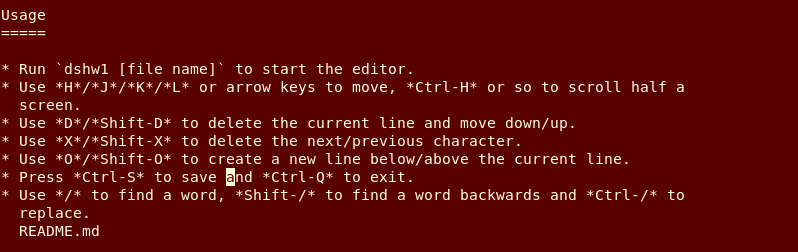
\includegraphics[height=3cm]{overview.png}
\end{center}

\subsection{项目特色}
该项目的大部分操作都模仿Vim来实现,但是有一些创新:
\begin{itemize}
	\item{} 借鉴GUI编辑器的一些特点,没有:开头的命令模式,使用快捷键Ctrl + S保存文件、Ctrl + Q退出
	\item{} 同样借鉴GUI编辑器的特点,查找替换等操作需要的参数在底部分行提示输入,类似GUI中的对话框
	\item{} 简化按键序列,没有两个键以上才需要完成的操作
	\item{} 光标含义总是Vim中插入模式中的含义,且移到一行的行尾或者行首时,继续左右移会跳转到相邻行行首或行尾
\end{itemize}
更详细的内容请参见项目中的README.md。

\subsection{项目结构}
整个项目分为三个部分: container, editor 和 ui,其中 container 为底层的数据结构,editor负责中间层的逻辑处理,ui负责上层的终端界面显示。
editor 获得用户的输入,然后对container进行修改和查询,最后将结果返回到ui进行输出。

ui的处理由倪泽堃同学负责,editor模块由罗翔宇同学负责,container的编写由顾澄同学负责。

\subsection{文件说明}

\begin{center}
	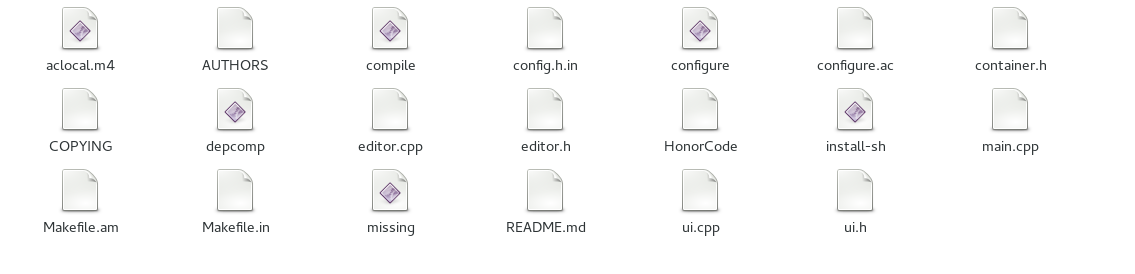
\includegraphics[height=3cm]{file.png}
\end{center}

\begin{itemize}
	\item{container.h:} 底层数据结构的声明和定义
	\item{editor.h, editor.cpp:} 声明并实现了一个类editor\_t,用于储存当前文件的内容和光标的状态
	\item{ui.h, ui.cpp:} 声明并实现了一个类ui\_t,包含了绘制界面、按键响应、模式切换等一系列界面交互所需要的函数
	\item{main.cpp:} 中间逻辑层的处理
	\item{HonorCode:} 诚实代码注释
	\item{README.md:} 项目README
	\item{COPYING, AUTHORS:} 项目许可证与作者
	\item{其它文件:} GNU Autotools生成的编译安装相关文件
\end{itemize}

\section{底层数据结构部分的分析与实现}
\subsection{分析}
一开始,我们组对于数据结构的选取有三个备选方案,分别为链表,平衡二叉树和块状链表,这三者各有优缺点。

其中链表的优点为,给定位置的插入和删除操作速度很快,可以达到 $O(1)$ 的时间复杂度,但是定位操作速度很慢,复杂度要降到 $O(n)$,其中 $n$ 为链表长度。

平衡二叉树的插入,删除和定位操作都很快,为对数时间复杂度,其中Splay树删除一段和插入一段也都能达到对数时间复杂度,若是可持久化Splay树,还能轻松实现撤销恢复功能。但是难于编写,代码量大。

而块状链表效率介于上面两者之间,其所有的操作均能在 $O(n^{0.5})$ 的时间内完成,其中 $n$ 为总字符数,但是编码也比较复杂。

经过反复的讨论和推敲,再考虑上实际的因素:时间过于仓促,而且这是一个小型编辑器很少会处理大型文件。我们一致认为应该将重点放在易于编写和易用之上,而不应改一味追求完美的时间复杂度。所以最终选择了使用链表来进行文件内容的储存。

\subsection{具体实现}
实质上该文本编辑器的底层是一个二维链表,其中第一维是用来储存行,而行链表中的每个元素都是一个字符链表,用于储存该行的字符。所以删除一行和插入一行就可以在行链表中进行操作,而且可以在常数时间内完成。删除和添加一个字符就可以在字符链表中进行操作,同样可以在常数时间内完成。

为了简化起见,我实现了一个模板类,方便代码的复用。类中维护了一个双向链表,方便插入和删除。

\subsection{链表域变量的说明}
\begin{itemize}
	\item{ch[0] \& ch[1]}

		使用一个长度为2的数组来表示下一个元素和上一个元素(ch[0]表示上一个,ch[1]表示下一个),而不是传统地开两个变量next和prev。这样,很多操作要求正向或者反向对链表进行操作时,都可以通过传一个表示方向的参数来完成,而不必实现两个几乎相同的函数。

	\item{null}

		一个空节点null来表示链表尾,而不是传统意义上的0x0来进行表示,这样省去了很多细节和边界条件的特判,方便代码的编写。

	\item{sum}

		由于tab的在实际显示中的长度不是固定的,所以链表中还额外维护了一个sum域,用于储存实际显示的长度。
\end{itemize}

\section{匹配算法的分析与实现}
\subsection{分析}
一开始,我们的备选方案有hash算法,后缀自动机和KMP算法,这三者各有利弊: 
\begin{itemize}
	\item{}其中hash算法最容易编写,而且时间复杂度也很优秀,为 $O(n+m)$,但是缺点是其正确率不能保证,有一定概率会出现错误。
	\item{} KMP算法比较容易编写,时间复杂度和hash算法相同,也为 $O(n+m)$,而且其算法流程对于链表保存的字符串有着天然的适用性。
	\item{} 后缀自动机比较难编写,但是其有着极其优秀的时间复杂度 $O(m)$,也就是其查找的时间复杂度只与模板串相关,与文本串的长度无关。但是最大的缺点在于,文本编辑器中的文本串是在不断变化中的,每次修改都要重构自动机花费太大。
\end{itemize}
经过一番讨论之后,我们最终选择使用KMP算法来实现查找和替换。

\subsection{实现}
KMP算法的实现还是比较简单的,但是与传统字符串中的KMP算法不同是,这里的next数组中元素不再是一个数,而是一个指针,指向链表中的对应元素。除此之外,就和普通的KMP算法毫无差别了。

在完成查找之后,利用链表的插入和删除操作即可完成文本的替换。

\section{界面部分的分析与实现}
\subsection{界面绘制}
在UNIX/Linux系统中,终端文本绘制、前景背景色设置、光标移动都是通过向stdout输出一些字符实现的,而按键响应则可以将stdin设置为non canonical模式后,用getchar函数读取。不过问题在于特殊键如方向键、退格键等等的键值是一个特定字符序列;控制光标位置、字符颜色等也需要输出一个特定字符序列。这些字符序列在每个终端不一定一样,需要读取terminfo后分析。于是我选取了一个易用的跨平台库ncurses来完成这个任务。这个库提供了一些简单的接口函数用于界面绘制,并且每次刷新界面时,ncurses都能智能地用尽量少的移动输出操作完成。

每次刷新界面时,绘制流程为:若刷新文本区域,则先从editor\_t底层类中获取显示区域的文本内容,再重新绘制文本区域。然后绘制状态栏。如果处于参数输入模式,还要绘制参数输入区域。

\vspace{1em}
\subsection{模式划分与切换、按键响应}
类似Vim,编辑器的模式一共划为普通模式、插入模式和参数输入模式。其中普通模式下用户可以移动光标、插入删除行与删除字符、查找替换保存退出等;插入模式和一般的GUI编辑器没什么不同;参数输入模式主要是用于查找替换保存时所需有关参数(查找词、保存文件名等)的输入。每一种模式都有自己的按键规则和响应函数。函数内调用底层editor\_t类的函数进行底层修改。函数执行完毕后,根据界面的修改情况刷新屏幕。

另外为了显示错误信息,类中还有一个变量储存错误的类型。若出现错误,则设置该变量。刷新屏幕显示错误后该变量置零,以使下一次操作后错误消息消失。

\vspace{1em}
\subsection{主程序与ui\_t类的交互}
主程序首先初始化界面,初始化ui\_t类,然后侦测用户按键并根据当前模式调用ui\_t类的相关函数。必要时函数会回传按键后所处的模式。主程序还设置了一个SIGWINCH信号的处理函数,当窗口大小发生变化时,会调用相关函数重绘界面。

\newpage
\section{统计数据}
该项目从9.19日开始进行,于10.12日结束, 共计 $49$ 次commits。以下是开发过程中每天的commits统计图:

\begin{center}
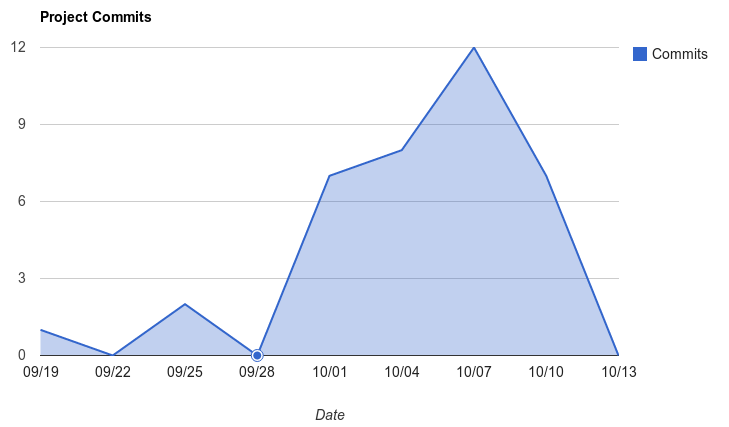
\includegraphics[height=6cm]{commits.png}
\end{center}

该项目有两个分支master和dev,采用git工具进行分支管理,应采取经典的git开发模式。日常的开发和测试在dev分支上进行,待调试通过后,将dev分支合并至master分支, 保证master分支始终是可用的稳定版本。

以下是各人分模块开发及合并示意图:
\vspace{1.5em}
\begin{center}
	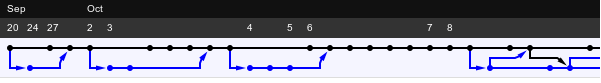
\includegraphics[height=1.1cm]{branch1.png}
	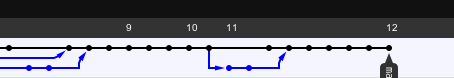
\includegraphics[height=1.1cm]{branch2.png}
\end{center}

\vspace{2em}
\section{心得体会}
这次大作业是我们第二次接触大型工程项目的开发。由于有了第一次的经验,我们这次在工具的选择和分工协作方面都分配得比较合理,给每个人分配了自己最擅长的工作,使大家都能充分发挥自己的长处,提高工作效率。

但是开发过程还是遇到很多困难和挑战的。比如对于文本编辑器中tab的处理,由于tab是一个非固定长度的字符,所以每次都要遍历一次链表来获得真正的显示长度。后来倪泽堃同学提出可以在链表中维护一个sum域来减少遍历操作,经过我们的编写测试后,发现编辑器的效率的确有了很大的提升。

另外在完成大作业的过程中,我们学到了一些新工具的用法;了解了字符终端控制的原理;了解了实际工程的开发的流程和方式。这不仅对我们的思维方式进行了良好的训练,也对代码能力有了大大的提升。

\end{document}
